% ====================================================================
%+
% SECTION:
%    section-name.tex  % eg lenstimedelays.tex
%
% CHAPTER:
%    chapter.tex  % eg cosmology.tex
%
% ELEVATOR PITCH:
%    Explain in a few sentences what the relevant discovery or
%    measurement is going to be discussed, and what will be important
%    about it. This is for the browsing reader to get a quick feel
%    for what this section is about.
%
% COMMENTS:
%
%
% BUGS:
%
%
% AUTHORS:
%    Phil Marshall (@drphilmarshall)  - put your name and GitHub username here!
%-
% ====================================================================

\section{Supernova Cosmology and Physics}
\def\secname{supernovae}\label{sec:\secname}
% \label{sec:cosmology, supernovae, classification, lenstimedelays, deepdrillingfields }

\noindent{\it Jeonghee Rho, Michelle Lochner, Rahul Biswas} % (Writing team)

% This individual section will need to describe the particular
% discoveries and measurements that are being targeted in this section's
% science case. It will be helpful to think of a ``science case" as a
% ``science project" that the authors {\it actually plan to do}. Then,
% the sections can follow the tried and tested format of an observing
% proposal: a brief description of the investigation, with references,
% followed by a technical feasibility piece. This latter part will need
% to be quantified using the MAF framework, via a set of metrics that
% need to be computed for any given observing strategy to quantify its
% impact on the described science case. Ideally, these metrics would be
% combined in a well-motivated figure of merit. The section can conclude
% with a discussion of any risks that have been identified, and how
% these could be mitigated.

This section is concerned with the detection, characterization of supernovae 
over time using the Large Synoptic Sky Telescope (LSST) and the use of these
supernovae for a number of science applications. The most important science 
application is the use of supernovae Type Ia (SNIa) and potentially some core-colapse SN (like Type IIP) to trace the recent expansion history of the universe,
and confront models of the physics driving the late time accelerated expansion
of the universe. 

This objective of supernova cosmology follows (at least for SNIa) several
highly successful surveys; improvement in that knowledge could come from
substantially larger numbers of well-characterized supernovae and potentially
useful redshift distributions of such detected supernovae. In this sense, this
goal is not directly tied to the large survey area that is an unprecedented
characteristic of the LSST. However, we shall argue that in practice, even this
goal would be largely helped by the spatial scale offered by the Wide Fast Deep
(WFD) component of the LSST. 

On the other hand, the WFD component of the LSST survey is potentially the 
first single survey to scan supernovae across the very large area of the
entire Southern sky. Therefore, supernovae detected and well characterized
(a) probing the isotropy of the universe, or (b) using peculiar velocities of 
supernovae to probe the growth of structure and finally (c) this may be the
best avenue for a highly complete sample of supernovae that will enable further
sharpening of our understanding of the properties of the supernova population 
of different types. 
This last point is extremely important for supernova cosmology goals: The success of supernova cosmology has always been based on the emperical model of intrinsic peak brightnesses being related to the certain observable characteristics of
supernovae. While the spatial location of the supernovae is not important, the 
WFD has the potential to dramatically increase the size of the sample 
available to train such an emperical model, as well understand the probability of deviations and scatter from this model. Aside from issues like calibration 
which need to be addressed differently, a larger sample size of such well measured supernovae is probably the only way to address deviations from the emperical
model usually discussed as `systematics'. This can be thought of in two 
components: the low redshift sample of supernovae which is more likely to be complete, and the higher redshift sample that might be able to constrain evolution. 
% --------------------------------------------------------------------

\subsection{Target measurements and discoveries}
\label{sec:keyword:targets}

% Describe the discoveries and measurements you want to make.

Supernovae of different types are visible over a time scale of about a few 
weeks (eg. Type Ia) to close to a year (Type IIP). During the full ten year
 survey of LSST, the telescope will scan the entire Southern Sky repeatedly
 with a universal Wide Fast Deep (WFD) Candence, and certain specific locations
of the sky called the Deep Drilling Fields (DDF) with special enhanced cadence. 

This spatio-temporal window should contain millions (RB: remember to check) of supernovae, that will have apparent magnitudes brighter than the single exposure limiting magnitude of LSST, for at least some time.  However, the actual
 sequence of observations in LSST defined by series of field pointings as a
 function of time in filter bands (along with weather conditions) will
 determine the extent to which each of such supernovae can be detected and
 characterized well.  Characterization of these supernovae is at the core of a
 number of science programs that use supernovae as bright, abundant objects with empirically determined intrinsic brightness. For LSST, this goal entails (a) detection of supernovae (b) photometric typing of supernovae, (c) estimating photometric redshifts of supernovae (or identifying host galaxies,
 and obtaining their redshifts from photometry or follow-up spectroscopy)
(c) estimation of intrinsic brightnesses of the supernovae, and finally use these data in addressing our science goals of cosmological inference, etc.
The efficacy of photometric typing, redshifts and estimation of intrinsic brightnesses are all
dependent on the amount of information available in the observed light curves of supernovae. While these steps are not necessarily independent, it is useful to think of the requirements on some of these steps separately; it is not unlikely  that combining some of these steps would still be affected by similar requirements. 

{\emph{Our first objective is to detect such supernovae}}. By `detection of supernovae', we mean a process
that detects transients from the subsets of LSST detection, and classify them as supernovae (as opposed to an AGN, or an asteroid). In brief, this process 
consists the identification of a set of image subtractions between high 
resolution `template` image of a sky section, and a set of single exposures at
different times (usually of lower resolution) of the same region, after 
attempting to correctly account for the different resolutions of images, and alignments. These sets of image subtractions associated
 with a single object will be used to detect the object as a transient and then
classify the transient as a supernova . Clearly, this step of detecting a supernova depends on the number of such images recorded per object, the number of filters and the signal to noise ratio of these images. One might expect that the efficiency of this step may be summarized as a threshold on the joint properties 
of an astrophysical candidate (apparent brightness, light curve characteristics, background) as well as observing conditions (Seeing etc.).  

{\emph{Our second objective is to photometrically classify different kinds of supernovae}} 
{\bfseries Photometric supernova classification}\\
In the past, only spectroscopically typed supernovae have been used for cosmology. Photometric 
typing from the light curve alone has only been used to select candidates for spectroscopic 
follow-up (see for example \citet{Sako2008}). However, LSST will simply produce far too many 
candidates for any chance of following up even a significant fraction of them. In order to avoid 
throwing away the majority of the supernova dataset, we need to use techniques capable of 
determining cosmological parameters from a potentially contaminated photometric supernova dataset.

There have been several techniques proposed in recent literature to solve this problem. One 
approach proposes applying stringent cuts to the photometric dataset to obtain a nearly pure sample 
of type Ia supernovae \citep{Bernstein2012,Campbell2013} and to run the standard supernova analysis 
with this sample. Another approach, BEAMS \citep{Kunz2007,Newling2011,Hlozek2012,Knights2013}, 
makes use of the full dataset, coping with contamination by using a mixture model for the 
likelihood, thus allowing for multiple populations. Whatever the technique ultimately used to for 
cosmological analysis, it will rely on accurate initial classifications of supernova type and 
unbiased estimates for the probability of each type.

The current state-of-the-art photometric classification techniques rely on fitting empirically 
determined templates of supernovae to light curves \citep{Jha2007,Guy2007,Sako2011}. However in 
recent years, new approaches have been published in response to the 2010 `Supernova 
Photometric Classification Challenge' \citep{Kessler2010a}. Many of these use novel light curve 
parameterisation and employ machine learning algorithms to perform the classification (see \citet{Kessler2010b} and references therein).

While many of these methods have been tested on standard sets of simulated data and (in some cases) 
on SDSS data, it is still not clear which technique (if any) is superior in all situations. For 
example, some techniques rely heavily on reliable redshift information being available, while others 
are less reliant on it. Some techniques may be more robust to non-representative datasets than 
others and it is not clear how the techniques will respond to changes in cadence, filter sets, SNR 
etc. With this in mind, we propose the use of a multifaceted classification system which employs 
several different methods of extracting features from the light curves (e.g. fitting parametric 
functions or templates) and several different classification algorithms. This system is highly 
modular, allowing the easy addition of new approaches for direct comparison with existing  techniques. This also allows direct analysis of different observing strategies, without having to 
make an initial choice of classification technique. 


{\emph{Our third obvective is to characterize supernovae in terms of emperical
    light curve models}}

The ultimate goal of using supernovae for a cosmology analaysis (either SNIa or SNIIP) requires an estimate of the intrinsic brightness of the supernova. The
first (and sometimes only step depending on the light curve model) to this, is
to fit the calibrated fluxes to a light curve model with a set of parameters.
According to the ansatz used in supernova cosmology, the intrinsic brightness of
 supernovae is largely determined by the parameters of the light curve model; 
 hence the uncertainties on the inferred parameters largely determine the
 uncertainties on the inferred peak intrinsic brightness or distance moduli of the supernovae.

% Now, describe their response to the observing strategy. Qualitatively,
% how will the science project be affected by the observing schedule and
% conditions? 

% In broad terms, how would we expect the observing strategy
% to be optimized for this science?





% --------------------------------------------------------------------

\subsection{Metrics}
\label{sec:keyword:metrics}

Quantifying the response via MAF metrics: definition of the metrics,
and any derived overall figure of merit.

\emph{To be added: discussion of the ROC curve as a useful metric for photometric supernova 
classification}

% --------------------------------------------------------------------

\subsection{OpSim Analysis}
\label{sec:keyword:analysis}

OpSim analysis: how good would the default observing strategy be, at
the time of writing for this science project?

As noted above the science goal of trying to characterize supernovae is largely
dependent on how well the light curves of individual supernovae are sampled in
time and filters. To study this, we reindex the opsim output on spatial
locations rather than use the temporal index. There are different methods (which will be merged), and here we will first illustrate this in terms the cadence in an example LSST field.

\begin{figure}
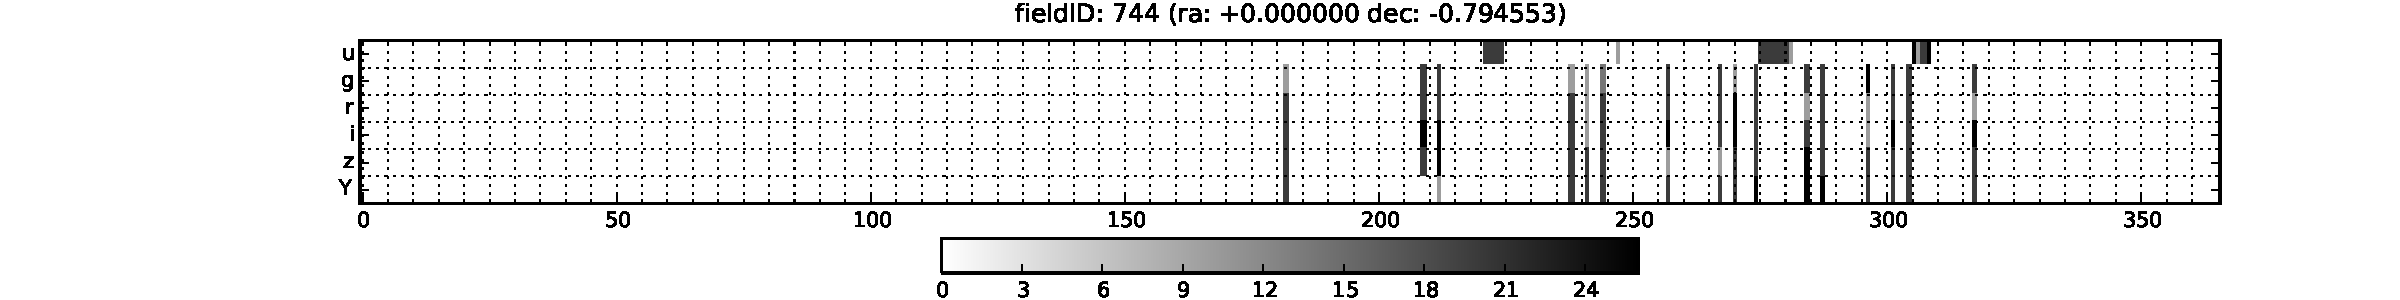
\includegraphics[width=\textwidth]{figs/supernova/fig_firstSeason_0}
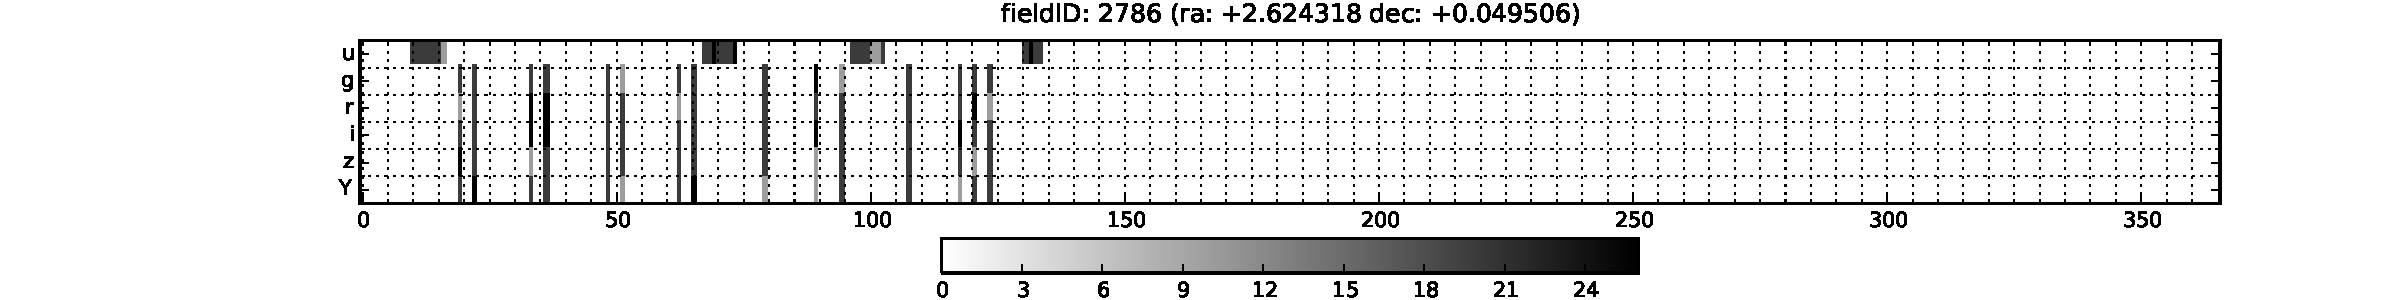
\includegraphics[width=\textwidth]{figs/supernova/fig_firstSeason_1}
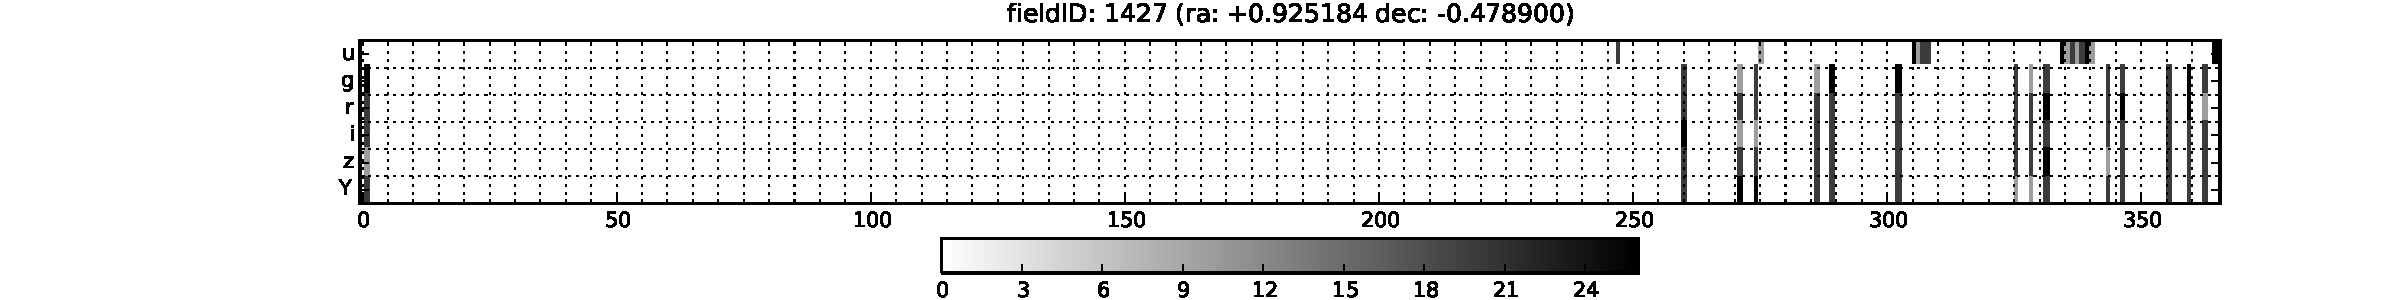
\includegraphics[width=\textwidth]{figs/supernova/fig_firstSeason_2}
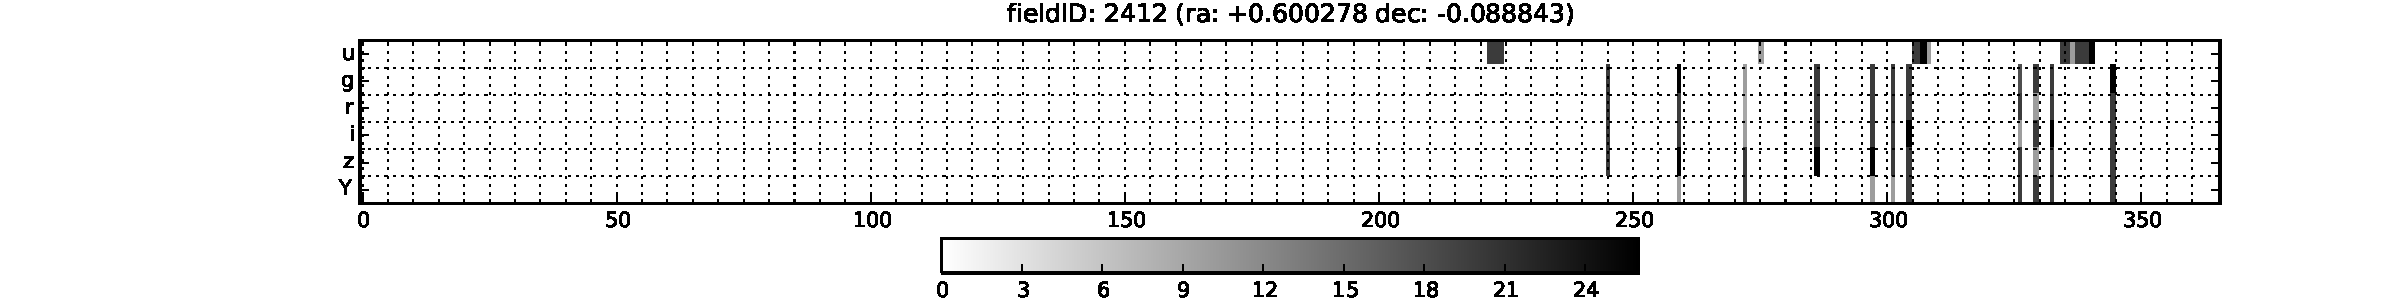
\includegraphics[width=\textwidth]{figs/supernova/fig_firstSeason_3}
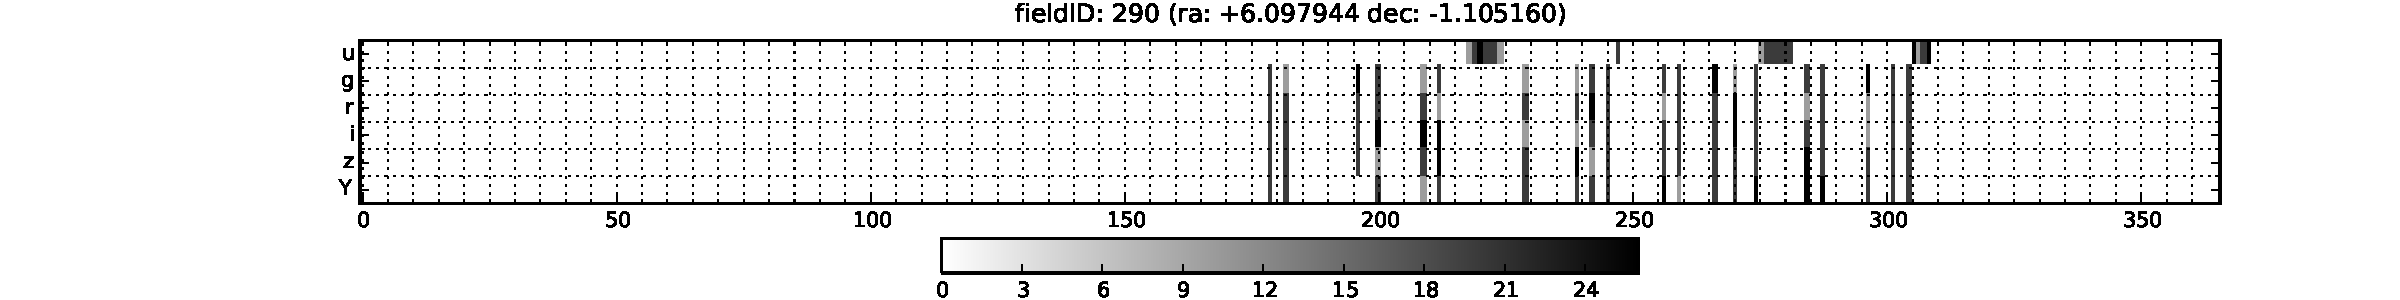
\includegraphics[width=\textwidth]{figs/supernova/fig_firstSeason_4}
\label{fig:opsimSummary}
\caption{Cadence in different filters for a few fields in the the ouptut
    of OpSim version Enigma 1189 .}
\end{figure}



% --------------------------------------------------------------------

\subsection{Discussion}
\label{sec:keyword:discussion}

Discussion: what risks have been identified? What suggestions could be
made to improve this science project's figure of merit, and mitigate
the identified risks?


\begin{itemize}
\item Intinsic Dispersion, environmental effects, newer analysis methods
\item Follow-up procedures: What is feasible? Where will our training samples for classification and light curve models come from (other experiments, our own 
sub-samples with spectroscopic follow-up), spectroscopic follow-up of host galaxies. Can hosts be identified?
\item `Systematics': In what ways will the real data not match the assumptions made in analysis
\end{itemize}


% ====================================================================

\navigationbar
